\section{Deep Learning Approach} \label{sec:build4}

Artificial Neural Networks\cite{ANN} shown in Figure \ref{fig:Figure20} was an idea conceived  in the 1960s to mimic the functions of the human brain in the way it absorbs information and learns from it. in order to  convert the whole notion into reality it took a lot more time than expected. The primary reason behind the delay is that back then, the computers were not powerful enough, the other reasons being the researchers were not totally aware of the problem. Then in 1986, eminent neural network researcher and computer scientist Dr. Geoffrey Hinton came up with the idea of backpropagation\cite{backpropagation} where a Deep Neural Network could be trained discriminatively and the weight updates can be done via stochastic gradient descentusing the following equation.

\begin{center}
	$w_{ij}(t+1) = w_{ij}(t) + \eta \frac{\partial C}{\partial w_{ij}}$
\end{center}
where $\eta$ s the learning rate, C is the cost function. The choice of the cost function depends on factors such as learning type whether it be supervised, unsupervised or reinforcement learning. 

\begin{figure}[t]
	\DeclareGraphicsExtensions{.pdf,.png,.jpg}
	\begin{center}
		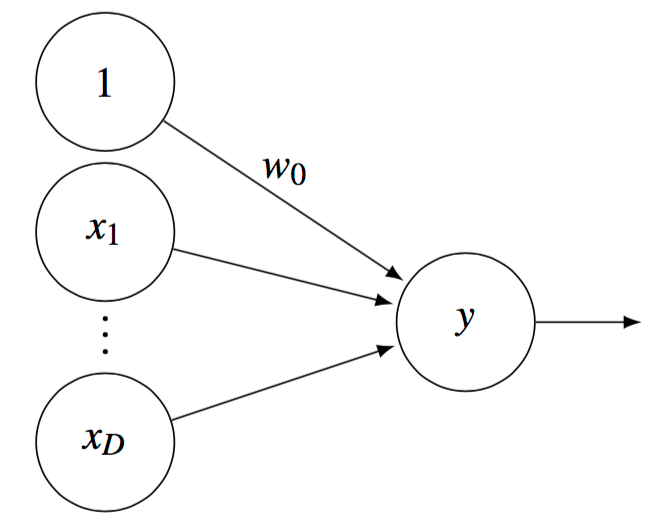
\includegraphics[width=0.7\textwidth]{Figures/Figure20}
	\end{center}
	\caption{Artificial Neural Network with D input neurons and 1 output neuron} 
	\label{fig:Figure20}
\end{figure}


The ability of multi-layer backpropagation networks has enabled the machines to learn complex high-dimensional non-linear mappings from large collections of example data which makes it obvious for visual recognition. In this method, rather than hand-crafting the various features, a raw image is first convoluted with a filter to find various feature maps. The feature maps are then connected together to form a fully-connected layer, the input of one layer is fed as the output of the next layer to create a deep network. The whole process rely on backpropagation to turn the first few layers into an appropriate feature extractor. Deep learning has achieved a lot of successes in the past for character recognition, digit recognition and recent works show that it is being applied to most topics of image representation and learning purposes. Just recently it has been applied to Face Recognition by training with lots of face image data and tremendous success has been reported[deep face paper].

The whole process of deep Convolutional Neural Networks(CNN)\cite{cnn} is very complex and requires a lot of computation to train and as a matter of fact, parallel computing is being brought forward to decrease the training time. The fully connected layer has several hundred hidden units and each of these units have specific weights assigned to them with the help of the back-propagation algorithm. Overfitting occurs if training data is scarce. Before being connected to the fully-connected neural network, the images need to be size normalized and centered in input fields. CNNs force the extraction of certain local features rather than global features which are obtained by hand-crafted feature extractors. LeCunn et al.\cite{lecun} have worked in digit recognition and have received tremendous success on digit recognition.

Deep Learning research stopped even after all these breakthroughs because the computers took a lot of time to train the large neural nets and at the same time a lot of image data was also not available. Researchers thought that it is better to go ahead with hand-crafted feature extractors which were giving better results at that time and took less time for computation. In 2006, Geoffrey Hinton and Ruslan Salakhuditnov worked on reducing the dimension of the data with neural networks in thier paper\cite{dbn}. Since then a lot of work has been done as computers have become powerful with the advent of modern parallel processing algorithms. One of the major breakthroughs came in 2012, when Alex Krizhevsky\cite{krizhevsky} build a huge neural network by training 15 million images from Imagenet\cite{imagenet} Database and then using Deep CNN they got one of the best result in the ImageNet competition for Image recognition and got a result which  was nearly 11 p.c. better than the second best approach which was done with SIFT + Fisher Vectors \cite{siftfisher}. Since then in the last 4 years quite a good amount of work has been done in this field. Several deep learning frameworks have been designed by researchers for researchers to move the work ahead - Some of the famous Frameworks being Caffe\cite{caffe} by University of California, Berkeley, Theano\cite{theano} by University de Montreal, TensorFlow\cite{tensorflow} by Google, Torch\cite{torch} and many others.

In our project we have used the Caffe Deep Learning Framework\cite{caffe} for our purposes. The reason we choose Caffe is being described below:

Caffe provides multimedia scientists and practitioners with a clean and modifiable framework for state of the art deep learning algorithms. It has a big collection of reference CNN models, it is licensed with BSD and is written in C++ and Python. Caffe can process upto 40 million images a day on a single NVIDIA K40. Caffe is maintained by Berkeley Vision and Learning Center(BVLC). Caffe makes it easy for users to build CNNs in their .prototxt file and also has several functions to draw networks and optimize them. It provides Pre-Trained models which is not provided by many of its competetitors. Caffe stores nd communicates data in 4-arrays called blobs for faster processing. Blobs provide a unified memory interface, holding batches of images , parameters or parameters updates. Blobs conceal the mental and mental overhead of mixed CPU/GPU operation by synchronizing from the CPU host to the CPU device as needed. 

A key problem in multimedia data analysis is discovery of effective representations for sensory inputs—images, sound- waves, haptics, etc. While performance of conventional, handcrafted features has plateaued in recent years, new developments in deep compositional architectures have kept performance levels rising \cite{krizhevsky}. Deep models have outperformed hand-engineered feature representations in many do- mains, and made learning possible in domains where engineered features were lacking entirely.
We are particularly motivated by large-scale visual recognition, where a specific type of deep architecture has achieved a commanding lead on the state-of-the-art. These Con-volutional Neural Networks, or CNNs, are discriminatively trained via back-propagation through layers of convolutional filters and other operations such as rectification and pooling. Following the early success of digit classification in the 90’s, these models have recently surpassed all known methods for large-scale visual recognition, and have been adopted by industry heavyweights such as Google, Facebook, and Baidu for image understanding and search.

While deep neural networks have attracted enthusiastic interest within computer vision and beyond, replication of published results can involve months of work by a researcher or engineer. Sometimes researchers deem it worthwhile to release trained models along with the paper advertising their performance. But trained models alone are not sufficient for rapid research progress and emerging commercial applications, and few toolboxes offer truly off-the-shelf deployment of state-of-the-art models—and those that do are often not computationally efficient and thus unsuitable for commercial deployment.

Caffe has several advantages over its peers. Caffe provides a complete toolkit for training, testing, finetuning, and deploying models, with well-documented examples for all of these tasks. As such, it’s an ideal starting point for researchers and other developers looking to jump into state-of-the-art machine learning. At the same time, it’s likely the fastest available implementation of these algorithms, making it immediately useful for industrial deployment.

Some of the main features of Caffe are:\\
\textbf{Modularity:} The software is designed from the begin- ning to be as modular as possible, allowing easy extension to new data formats, network layers, and loss functions. Lots of layers and loss functions are already implemented, and plentiful examples show how these are composed into train- able recognition systems for various tasks. \\

 \textbf{Separation of representation and implementation:} Caffe model definitions are written as config files using the Protocol Buffer language. Caffe supports network archi- tectures in the form of arbitrary directed acyclic graphs. Upon instantiation, Caffe reserves exactly as much memory as needed for the network, and abstracts from its underly- ing location in host or GPU. Switching between a CPU and GPU implementation is exactly one function call. \\

\textbf{Test coverage:} Every single module in Caffe has a test, and no new code is accepted into the project without corre- sponding tests. This allows rapid improvements and refac- toring of the codebase, and imparts a welcome feeling of peacefulness to the researchers using the code. \\

\textbf{Python and MATLAB bindings:} For rapid proto- typing and interfacing with existing research code, Caffe provides Python and MATLAB bindings. Both languages may be used to construct networks and classify inputs. The Python bindings also expose the solver module for easy pro- totyping of new training procedures.

\begin{figure}[t]
	\DeclareGraphicsExtensions{.pdf,.png,.jpg}
	\begin{center}
		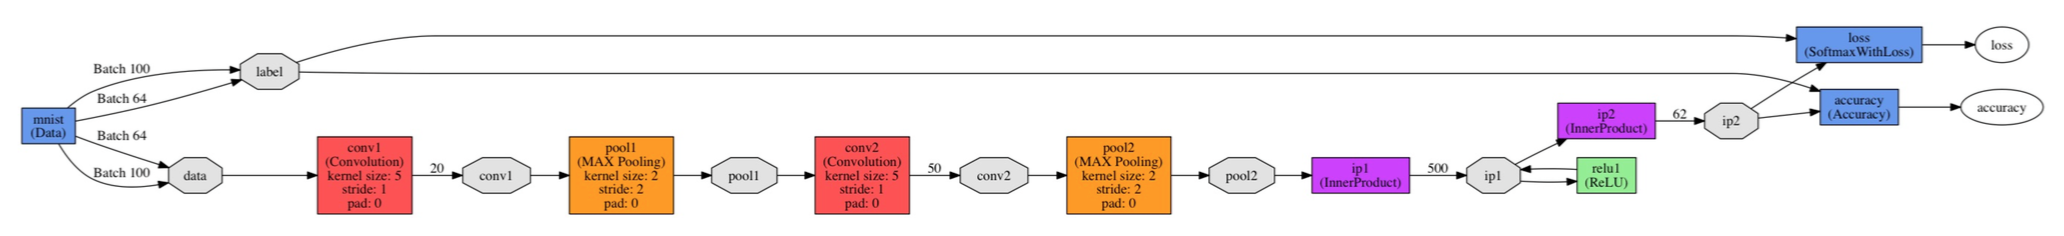
\includegraphics[width=\textwidth]{Figures/Figure18}
	\end{center}
	\caption{LeNet Network Diagram}
	\label{fig:Figure18}
\end{figure}
